\chapter{CryptDB as a Software}
\label{chp:software}

Although CryptDB is mainly a proof of concept rather than a commercial software, the source code is available along with instructions on how to install it. This chapter will cover the installation and setup of CryptDB's proxy server, how to connect the proxy server to a regular database system, and finally a small demo application will be presented.

\section{Installation of CryptDB's Software}

CryptDB comes as a software available through MIT, and can be downloaded using the version control system Git. As the creators has moved on to other projects, the source code has not been maintained since 2014, and is currently only tested on Ubuntu 12.04 and Ubuntu 13.04. During the installation of CryptDB, some issues has been encountered. Since CryptDB is only tested with said Ubuntu versions, the natural approach would be to install the software on one of the two Ubuntu versions. This often involves running some sort of \gls{vm} in some \gls{vmm}, which is very inconvenient when developing applications that should be able to run regardless of operating system and environment. When working inside a \gls{vm} installing and working with software that is at best ready for alpha testing, you better watch your steps. 

\subsection{Docker to the Rescue}


Because of the presented reasons, some of the work related to this project has been to detach CryptDB from such requirements and providing a workable environment regardless of operating system which is easy to restore if one were to corrupt the state if the system. Docker \cite{docker_homepage} is an open-source software allowing programs to be wrapped up in \emph{containers}. Containers are complete file systems containing every piece of code, 
library and dependency the program need to run properly, which runs directly on the host OS without the need of a \gls{vmm} and Guest OSs. After a container is built, it can be shipped and run in other environments such as Windows, OS X and Linux without issues or adjustments.

A guide on how to install and set up CryptDB's database and proxy server can be found in Appendix \ref{app:setup} along with a small introduction on how to play with the software as presented in Appendix \ref{app:playaround}.


\section{A Small Demo Application}

Along with the exploring of CryptDB, a tiny sample application has been developed in order to understand the sytem. The application allows a single user to maintain employee information for a fictive firm. As the software itself only supports applications running in the single-user mode, there has not been made any attempts in creating an application consisting of multiple users. The application is written in Python, which is a high-level programming language with a lot of functionality \cite{python}. In order to add database functionality to the application, MySQLdb is used as an interface to provide the MySQL API for Python \cite{mysqldb}.

\subsection{Database Server and Proxy Server}

CryptDB needs to have a database running in the background for the proxy server to connect to. As described in the previous section, Docker is used to set up a container hosting both the database and the CryptDB proxy. When connecting to a database, the user needs to specify a few parameters such as the address of the machine hosting the database server, user name, password, port number and the name of the database it wants to connect to. A regular MySQL database server runs on port \verb!3306!, while CryptDB's proxy server is programmed to listen for connections on port \verb!3307! and relay queries to the database server listening on port \verb!3306!. All this is taken care of by following the guide presented in Appendix \ref{app:setup}.

\subsection{Application for Storing Employee Records}

Figure \ref{fig:app_mm_user} shows the main menu when logging into the application. There are not many features implemented in the application, as the whole process of just getting CryptDB's software up and running was somewhat time consuming. It allows the user to display the list of employees along with their personal records, adding new employees, as well as updating them. It is mainly developed to test out functionality, therefore it also supports "free queries" where the user can perform queries directly to the proxy (or database). For navigating in the application, the user specifies commands by typing in their corresponding number.
\newpage
\begin{figure}[h]
	\centering
	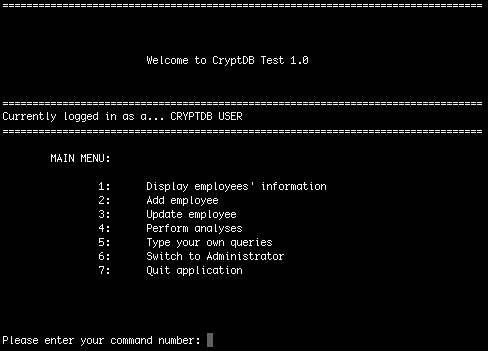
\includegraphics[scale=0.45]{terminal/app_user_mainmenu.png}
	\caption{Main menu for users logged in as CryptDB users, i.e. connecting through the proxy server.}
	\label{fig:app_mm_user}
\end{figure}

When the user selects option 1 in order to show information regarding the employees of the firm, the application sends a \verb!SELECT * FROM employees;! query to the proxy server. As previously explained, the proxy server intercepts the query and anonymizes it. This can be seen in Figure \ref{fig:proxy_enc_res}, which also shows the encrypted result that is returned from the database server. The result is then decrypted and sent to the application, where it is displayed to the user as seen in Figure \ref{fig:app_user_emp}.

\begin{figure}[h]
	\centering
	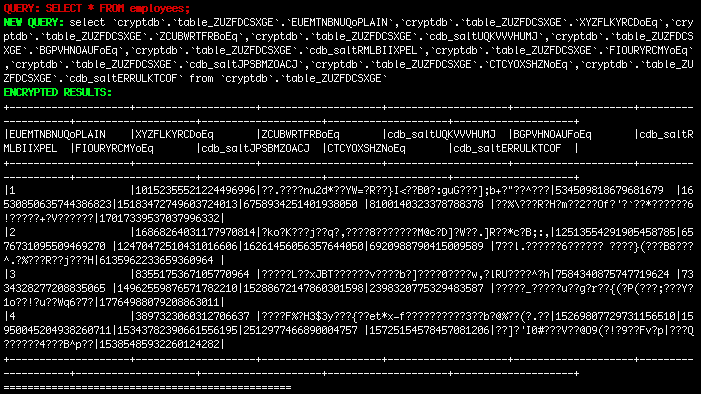
\includegraphics[scale=0.45]{terminal/proxy_enc_res.png}
	\caption{The observed processing at the proxy server when querying information about all employees.}
	\label{fig:proxy_enc_res}
\end{figure}


\begin{figure}[h]
	\centering
	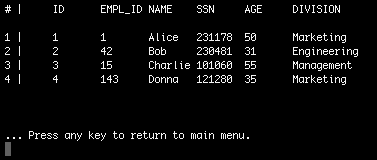
\includegraphics[scale=0.7]{terminal/app_user_emp.png}
	\caption{The result displayed at the CryptDB user when querying for information regarding all employees.}
	\label{fig:app_user_emp}
\end{figure}

\newpage

\subsection{Confirming the Encrypted Administrator View}

To illustrate the case of the curious database administrator, which is the most easy-to-demonstrate threat, the application has two views. These are the CryptDB user view, and the database administrator view, which can easily be switched between in the application. Depending on whether the application is connected through the proxy or not, the menu items also changes as shown in Figure \ref{fig:app_mm_user} and Figure \ref{fig:app_mm_admin}. Such a switch is performed by simply disconnecting from the application and perform a new log-in on either port 3306 or 3307 based on the previous view. The available menu items depends on the current user's role.

\begin{figure}[h]
	\centering
	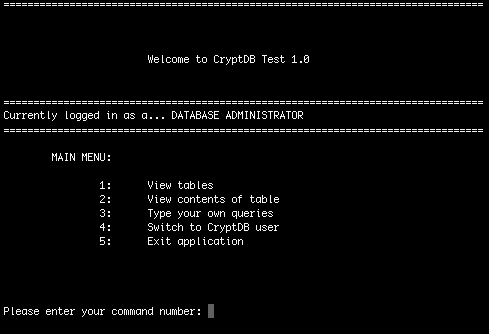
\includegraphics[scale=0.55]{terminal/app_admin_mainmenu.png}}
	\caption{Main menu for administrators, i.e. connecting directly to the database server.}
	\label{fig:app_mm_admin}
\end{figure}

\begin{wrapfigure}[14]{r}{8cm}
	\centering
    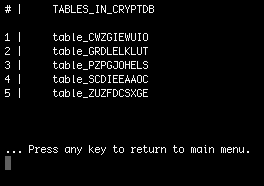
\includegraphics[scale = 0.75]{terminal/app_admin_enc_res1.png}
    \caption{Encrypted tables in CryptDB from a database administrator's perspective}
    \label{fig:app_admin_enc_res1}
\end{wrapfigure}
For curious database administrators, in addition to performing "free queries", they are also able to view the tables stored in the database, as well as displaying the contents of a table. Remember that one of the key features of CryptDB is that it protects against such curious administrators by encrypting all data inserted in the database.

Figure \ref{fig:app_admin_enc_res1} displays the result when querying the database with the \verb!SHOW TABLES;! statement. All table names are encrypted making it difficult for the administrator to achieve any knowledge about the database. One of the features in the administrator's view is to view the contents of a table, which is done by specifying the name of the table. While the data is encrypted, this does not prevent a curious to perform queries on the encrypted data. For example, there is no obstacles for him to perform a query such as

\begin{verbatim}
SELECT *
FROM table_ZUZFDCSXGE;
\end{verbatim}

But, the resulting data is of course encrypted, and shows nothing more than obscure symbols. Figure \ref{fig:admin_enc_res2} shows the resulting data to the query above. Note that the only property not to be encrypted is the row id, hence the database administrator is able to find out the number of rows in a table.

\begin{figure}[h]
	\centering
	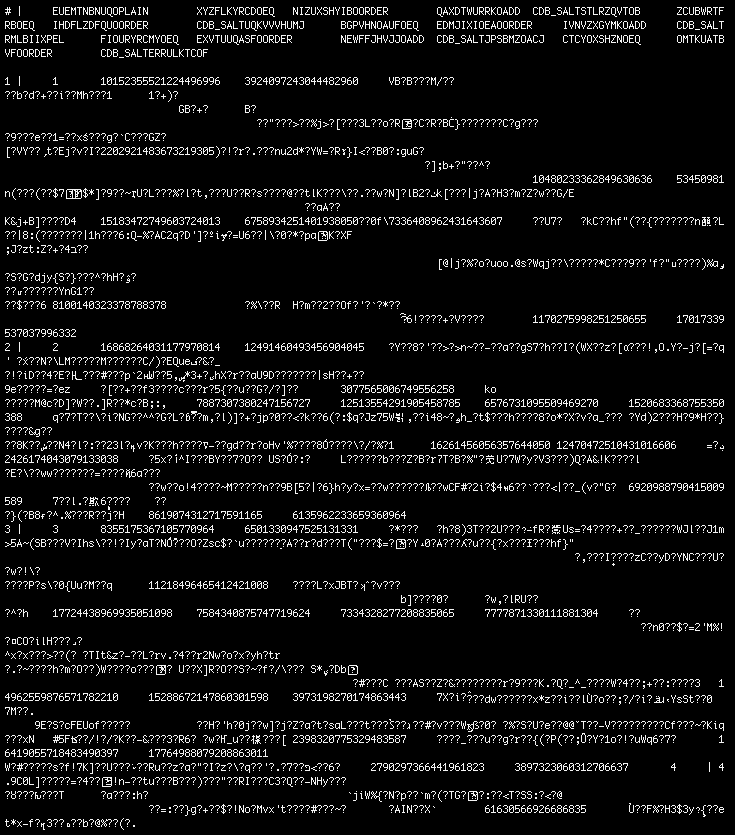
\includegraphics[scale=0.30]{terminal/app_admin_enc_res2.png}
	\caption{Encrypted data observed by the database administrator.}
	\label{fig:admin_enc_res2}
\end{figure}



\newpage
\subsection{Inspecting CryptDB Using DBMS Tools}

Python and MySQLdb does not provide any graphical way to investigate the database server. However, by installing a \gls{dbms} environment such as MySQL Workbench \cite{mysql_workbench}, inspecting the database suddenly becomes possible. MySQL Workbench provides many different features when inspecting databases, all from performing queries on the tables and describing tables and fields, to 
monitoring the database. By simply logging in, the administrator is able to view all tables in the database and inspect them by issuing the \verb!SELECT! query mentioned in the previous section.

\begin{figure}[h]
	\centering
	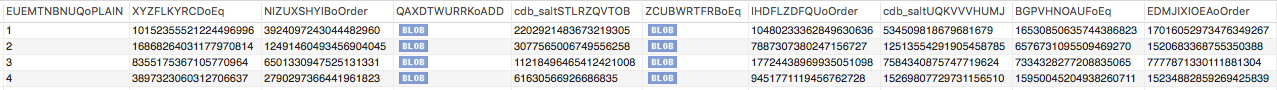
\includegraphics[scale=0.285]{terminal/admin_query_result.png}
	\caption{The resulting rows from performing a SELECT query on the encrypted table. Only the encrypted values of the two first columns is shown. \textbf{Should I show just one column instead so it is easier to see?}}
	\label{fig:admin_query_result}
\end{figure}

As observed, the data is not displayed as random symbols as from the demo application, but rather represented as large integers. It also possible to observe the different onion encryptions of each attribute as they are encrypted as separate columns. By looking very closely at the figure above, it is possible to spot the name of the columns, where the EQ-onion ends with \emph{eq}, the ORD-onion with \emph{Order} and the ADD-onion with \emph{ADD}. Figure \ref{fig:admin_fields_view} shows a clearer picture of the available information when inspecting tables. The database administrator is able to see the number of columns, and what type of onions the column is encrypted under.

\begin{figure}[h]
	\centering
	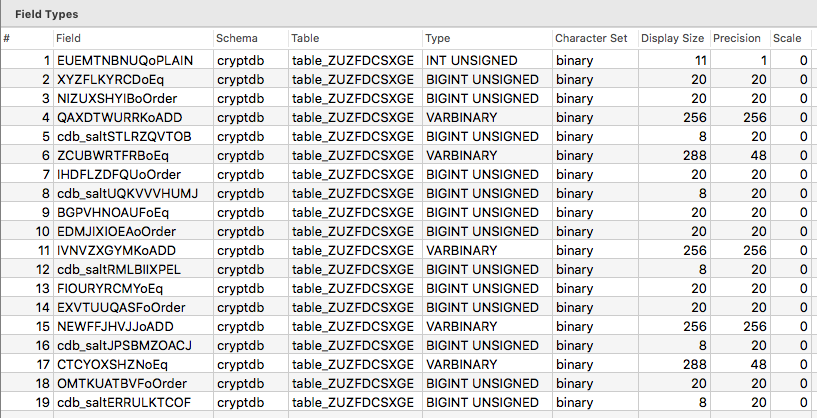
\includegraphics[scale=0.4]{terminal/admin_fields_view.png}
	\caption{Overview of the fields in the encrypted table table\_ZUZFDCSXGE when inspecting the database using MySQL Workbench.}
	\label{fig:admin_fields_view}
\end{figure}

\section{Discussion on CryptDB as a Software}

Should I just skip the discussion, perhaps? \\

While being a bit challenging to install and successfully connect to a database system, CryptDB seems to work as intended when operating on encrypted data. This project has not investigated the overhead when using CryptDB compared to a regular \gls{dmbs}, but the developers states that the throughput of CryptDB is 21-26\% lower than running on a regular MySQL server \citep{CryptDB_Main_Paper}. 

Something more...

The authors of CryptDB has taken the idea further with Mylar (\url{https://css.csail.mit.edu/mylar/}, which addresses the threat of attacks on multi-user mode. It is created with the experience from CryptDB in mind, but with focus on running web applications, which is one of the reasons that the multi-user mode has been deprecated from the latest versions of CryptDB.